
\documentclass[pdftex,11pt]{article}
\usepackage{marvosym}
\usepackage{comment}
\usepackage{url}
\usepackage{graphicx}
\usepackage{hyperref}
\usepackage{latexsym,amssymb}
\usepackage{amssymb,amsmath}
\usepackage{color}

\input{../../vrac/rgb.tex}
\input{../../vrac/env_python_listing.tex}


\usepackage[english]{babel}
\usepackage{array}
\usepackage{multirow} 

\hypersetup{
pdftitle={Langou :: Sauer EX.0.3.7 (answer)},
pdfauthor={Julien Langou}, 
} 

\setlength{\oddsidemargin}{-0.5in}
\setlength{\evensidemargin}{-0.5in}

\setlength{\textwidth}{7.4in}
\setlength{\textheight}{10.0in}

\setlength{\topmargin}{-0.75in}
\setlength{\headheight}{0pt}
\setlength{\headsep}{0pt}

\setlength{\parindent}{0pt}

\begin{document}

\thispagestyle{empty}
\pagestyle{empty}
\renewcommand{\theenumi}{\alph{enumi}}

\begin{center}
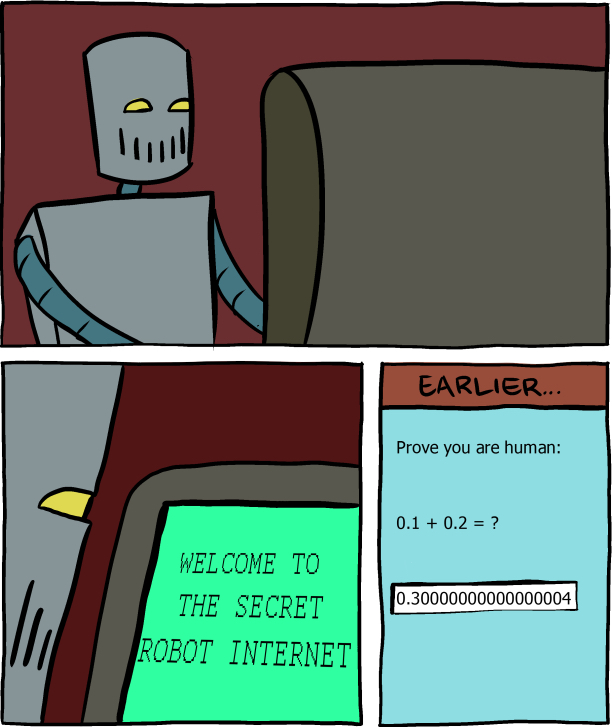
\includegraphics[width=0.5\textwidth]{meme_0_3.jpeg}
\end{center}

\vspace*{.7cm}

\framebox{
\begin{minipage}{\textwidth}
{\tiny
{\bf Copyright (c) 2021, Julien Langou. All rights reserved,}
please visit \url{https://creativecommons.org/licenses/by/4.0/}.}
\end{minipage}}
\vspace*{.2cm}


To understand the meme, just type in Python

\begin{python}
0.1 + 0.2
\end{python}
\begin{pythonoutput}
0.30000000000000004
\end{pythonoutput}

And then, well, obviously $$0.1+0.2 = 0.3,$$ so it seems weird that a computer returns 
$0.30000000000000004$ while the answer is ``obviously'' (for us humans) $0.3$.\\


\vspace*{.2cm}

Here is an explanation. 

We did the 64-bit floating-point machine number representation of $0.1$ and $0.2$ in EX.0.3.7 
(see \href{http://math.ucdenver.edu/~langou/4650/0.3/exercise_ex_0_3_07________sauer____sol_langou/exercise_ex_0_3_07________sauer____sol_langou.pdf}{url}), 
and we saw that, in a 64-bit floating point IEEE system, 0.1 and 0.2 are stored
as the machine numbers, respectively as: 
\begin{eqnarray}
 \nonumber \textmd{fl}(0.1)       & = &  + 2^{-4} ( 1.1001100110011001100110011001100110011001100110011010)_2~~\textmd{\scriptsize\color{blue}\# this is a machine number}\\
 \nonumber \textmd{fl}(0.2)       & = &  + 2^{-3} ( 1.1001100110011001100110011001100110011001100110011010)_2~~\textmd{\scriptsize\color{blue}\# this is a machine number}
\end{eqnarray}

If we prefer to see this in base 10:
\begin{eqnarray}
 \nonumber \textmd{fl}(0.1)       & = &  0.1000000000000000055511151231257827021181583404541015625~~\textmd{\scriptsize\color{blue}\# this is a machine number}\\
 \nonumber \textmd{fl}(0.2)       & = &  0.2000000000000000111022302462515654042363166809082031250~~\textmd{\scriptsize\color{blue}\# this is a machine number}
\end{eqnarray}
(Base 10 is not really useful. Base 2 is just fine. But base 10 might help for comprehension.) 


Then, we do (in exact arithmetic) the base-two addition, $x = \textmd{fl}(0.1) + \textmd{fl}(0.2)$, and we get
$$
\begin{array}{ccl}
  & 2^{-4}( \phantom{11}1.1001100110011001100110011001100110011001100110011010 )_2 & \textmd{\scriptsize\color{blue}\# this is fl(0.1), this is a machine number} \\
+ & 2^{-4}( \phantom{1}11.0011001100110011001100110011001100110011001100110100 )_2 & \textmd{\scriptsize\color{blue}\# this is fl(0.2), this is a machine number} \\
\hline
  & 2^{-4}(           100.1100110011001100110011001100110011001100110011001110 )_2 & \textmd{\scriptsize\color{blue}\# this is x = fl(0.1) + fl(0.2)}\\
  &                                                                                & \textmd{\scriptsize\color{blue}\# this is not a machine number }
\end{array}
$$

So in other words
\begin{eqnarray}
 \nonumber x = \textmd{fl}(0.1)+\textmd{fl}(0.2)       & = &  + 2^{-2} ( 1.001100110011001100110011001100110011001100110011001110 )_2 
\end{eqnarray}
$x$ is not a machine number. We cannot store $x$ exactly on the computer since
$x$ has 55 bits in the scientific notation. And we can only store 53 bits: 1
hidden bit and 52 mantissa bits.\\


We can do the same addition in base 10. (This is not really useful. Base 2 is just fine. But base 10 might help for comprehension.)
$$
\begin{array}{ccl}
  & 0.1000000000000000055511151231257827021181583404541015625 & \textmd{\scriptsize\color{blue}\# this is fl(0.1), this is a machine number} \\
+ & 0.2000000000000000111022302462515654042363166809082031250 & \textmd{\scriptsize\color{blue}\# this is fl(0.2), this is a machine number} \\
\hline
  & 0.3000000000000000166533453693773481063544750213623046875 & \textmd{\scriptsize\color{blue}\# this is x = fl(0.1) + fl(0.2)}\\
  &                                                                                & \textmd{\scriptsize\color{blue}\# this is not a machine number }
\end{array}
$$


Now, $x = ( \textmd{fl}(0.1) + \textmd{fl}(0.2) )$ is stored in the computer as the machine number 
$\textmd{fl}(x) = \textmd{fl}( \textmd{fl}(0.1) + \textmd{fl}(0.2) )$. 
$\textmd{fl}(x)$ will either be $x_-$, the machine number just smaller than $x$; or $x_+$, the machine number just bigger than $x$.

$$
\begin{array}{lcll}
 \nonumber x_-  & = &  + 2^{-2} ( 1.0011001100110011001100110011001100110011001100110011\phantom{|10}~~~)_2&\textmd{\scriptsize\color{blue}\# this is a machine number} \\
 \nonumber x    & = &  + 2^{-2} ( 1.0011001100110011001100110011001100110011001100110011|10~~~)_2          &\textmd{\scriptsize\color{blue}\# this is not a machine number} \\
 \nonumber x_+  & = &  + 2^{-2} ( 1.0011001100110011001100110011001100110011001100110100\phantom{|10}~~~)_2&\textmd{\scriptsize\color{blue}\# this is a machine number}
\end{array}
$$




We need to take the machine numbers $x_-$ or $x_+$ whichever is closer from
$x$. But we see that $x$ is right in the middle of $x_-$ and $x_+$. Dang it!
\Smiley.  Right in the middle. So then we use the ``ties to even'' rule: ``if
the number falls midway, it is rounded to the nearest value with an even least
significant digit.'' (Please note that since $x_-$ and $x_+$ are two
consecutive machine numbers, the last bit of one of two must be a 0, while last
bit of the other must be a 1. The rule says: ``pick the one with the last bit a
0''.) The 52-nd bit of $x_-$ is 1. The 52-nd bit of $x_+$ is 0. So, then, we
round $x$ is $x_+$. So $\textmd{fl}(x)$ is $x_+$. So we get:


$$\textmd{fl}( \textmd{fl}(0.1) + \textmd{fl}(0.2) ) = + 2^{-2} ( 1.0011001100110011001100110011001100110011001100110100 )_2  $$

We can also look at $x_-$, $x$, and $x_+$ in base 10. We get
$$
\begin{array}{lcll}
 \nonumber x_-  & = &  0.299999999999999988897769753748434595763683319091796875   &\textmd{\scriptsize\color{blue}\# this is a machine number} \\
 \nonumber x    & = &  0.3000000000000000166533453693773481063544750213623046875  &\textmd{\scriptsize\color{blue}\# this is not a machine number} \\
 \nonumber x_+  & = &  0.3000000000000000444089209850062616169452667236328125000  &\textmd{\scriptsize\color{blue}\# this is a machine number}
\end{array}
$$

So that 
$$\textmd{fl}( \textmd{fl}(0.1) + \textmd{fl}(0.2) ) = 0.3000000000000000444089209850062616169452667236328125000  $$


We can quickly check all this in python with

\begin{python}
import struct
print(f"{struct.unpack('<Q',struct.pack('<d',( 0.1 + 0.2 )))[0]:#066b}")
\end{python}
\begin{pythonoutput}
0b0011111111010011001100110011001100110011001100110011001100110100
\end{pythonoutput}

We remove the \texttt{0b} at the start and are left with the 64 bits.
Breaking the 64 bits with 1 bit (sign), 11 bits (exponent) and 52 bits (mantissa), this reads:
$$
0~|~01111111101~|~0011001100110011001100110011001100110011001100110100 
$$
The first bit \texttt{0} represents the sign +. $\checkmark$
The next 8 bit bit \texttt{01111111101} represents the exponent $-2$, 
We have that $(01111111101)_2 = 1021$ and then 
$1021-1023 = -2$, so we find that the exponent is $-2$. $\checkmark$
The last 52 bits \texttt{0011001100110011001100110011001100110011001100110100} 
is the mantissa, they represent $(1.0011001100110011001100110011001100110011001100110100)_2$.  $\checkmark$\\

And here you go. This is why when we type
\begin{python}
0.1 + 0.2
\end{python}
we get
\begin{pythonoutput}
0.30000000000000004
\end{pythonoutput}

Fun!

\vspace*{1cm}
\underline{Note:} I used \pythoninline{mpmath} for extended precision accuracy for the following computations.
The goal was to obtain the exact base-10 representation of numbers. This is not needed in practice but base-10 might help for some understanding.
\begin{python}
from mpmath import *
mp.dps = 100

# In base 10, fl( 0.1 ) is
print("fl(0.1)                 = ", mpf(2**(-4)*(  2**(  0) + 2**( -1) + 2**( -4) + 2**( -5) + 2**( -8) + 2**( -9) + 2**(-12) + 2**(-13) + 2**(-16) + 2**(-17)
         + 2**(-20) + 2**(-21) + 2**(-24) + 2**(-25) + 2**(-28) + 2**(-29) + 2**(-32) + 2**(-33) + 2**(-36) + 2**(-37)
         + 2**(-40) + 2**(-41) + 2**(-44) + 2**(-45) + 2**(-48) + 2**(-49) + 2**(-51) )))

# In base 10, fl( 0.2 ) is
print("fl(0.2)                 = ", mpf(2**(-3)*(  2**(  0) + 2**( -1) + 2**( -4) + 2**( -5) + 2**( -8) + 2**( -9) + 2**(-12) + 2**(-13) + 2**(-16) + 2**(-17)
         + 2**(-20) + 2**(-21) + 2**(-24) + 2**(-25) + 2**(-28) + 2**(-29) + 2**(-32) + 2**(-33) + 2**(-36) + 2**(-37)
         + 2**(-40) + 2**(-41) + 2**(-44) + 2**(-45) + 2**(-48) + 2**(-49) + 2**(-51) )))

# In base 10, fl(0.1) + fl( 0.2 ) is
print("fl(0.1) + fl(0.2)       = ", mpf(2**(-4)*(  2**(  0) + 2**( -1) + 2**( -4) + 2**( -5) + 2**( -8) + 2**( -9) + 2**(-12) + 2**(-13) + 2**(-16) + 2**(-17)
         + 2**(-20) + 2**(-21) + 2**(-24) + 2**(-25) + 2**(-28) + 2**(-29) + 2**(-32) + 2**(-33) + 2**(-36) + 2**(-37)
         + 2**(-40) + 2**(-41) + 2**(-44) + 2**(-45) + 2**(-48) + 2**(-49) + 2**(-51) )) 
         + mpf(2**(-3)*(  2**(  0) + 2**( -1) + 2**( -4) + 2**( -5) + 2**( -8) + 2**( -9) + 2**(-12) + 2**(-13) + 2**(-16) + 2**(-17)
         + 2**(-20) + 2**(-21) + 2**(-24) + 2**(-25) + 2**(-28) + 2**(-29) + 2**(-32) + 2**(-33) + 2**(-36) + 2**(-37)
         + 2**(-40) + 2**(-41) + 2**(-44) + 2**(-45) + 2**(-48) + 2**(-49) + 2**(-51) )))

# In base 10, fl( fl( 0.1 ) + fl( 0.2 ) ) is
print("fl( fl(0.1) + fl(0.2) ) = ", mpf(2**(-2)*(  2**(  0) + 2**( -3) + 2**( -4) + 2**( -7) + 2**( -8) + 2**(-11) + 2**(-12) + 2**(-15) + 2**(-16) + 2**(-19) + 2**(-20)
                  + 2**(-23) + 2**(-24) + 2**(-27) + 2**(-28) + 2**(-31) + 2**(-32) + 2**(-35) + 2**(-36) + 2**(-39) + 2**(-40)
                  + 2**(-43) + 2**(-44) + 2**(-47) + 2**(-48) + 2**(-50) )))
\end{python}
\begin{pythonoutput}
fl(0.1)                 =  0.1000000000000000055511151231257827021181583404541015625
fl(0.2)                 =  0.200000000000000011102230246251565404236316680908203125
fl(0.1) + fl(0.2)       =  0.3000000000000000166533453693773481063544750213623046875
fl( fl(0.1) + fl(0.2) ) =  0.3000000000000000444089209850062616169452667236328125
\end{pythonoutput}


\begin{comment}
\underline{Note:} I used \url{https://keisan.casio.com/calculator} for extended precision accuracy for the following computations.
The goal was to obtain the exact base-10 representation of numbers. This is not needed in practice but base-10 might help for some understanding.
\footnotesize
\begin{verbatim}
# In base 10, fl( 0.1 ) is
2^(-4)*(  2^(  0) + 2^( -1) + 2^( -4) + 2^( -5) + 2^( -8) + 2^( -9) + 2^(-12) + 2^(-13) + 2^(-16) + 2^(-17)
        + 2^(-20) + 2^(-21) + 2^(-24) + 2^(-25) + 2^(-28) + 2^(-29) + 2^(-32) + 2^(-33) + 2^(-36) + 2^(-37)
        + 2^(-40) + 2^(-41) + 2^(-44) + 2^(-45) + 2^(-48) + 2^(-49) + 2^(-51) )
=> 0.1000000000000000055511151231257827021181583404541015625

# In base 10, fl( 0.2 ) is
2^(-3)*(  2^(  0) + 2^( -1) + 2^( -4) + 2^( -5) + 2^( -8) + 2^( -9) + 2^(-12) + 2^(-13) + 2^(-16) + 2^(-17)
        + 2^(-20) + 2^(-21) + 2^(-24) + 2^(-25) + 2^(-28) + 2^(-29) + 2^(-32) + 2^(-33) + 2^(-36) + 2^(-37)
        + 2^(-40) + 2^(-41) + 2^(-44) + 2^(-45) + 2^(-48) + 2^(-49) + 2^(-51) )
=> 0.2000000000000000111022302462515654042363166809082031250

# In base 10, x = fl( 0.1 ) + fl( 0.2 )
   0.1000000000000000055511151231257827021181583404541015625
+  0.2000000000000000111022302462515654042363166809082031250
=> 0.3000000000000000166533453693773481063544750213623046875

# In base 10, fl( fl( 0.1 ) + fl( 0.2 ) ) (which is x+) is
2^(-2)*(  2^(  0) + 2^( -3) + 2^( -4) + 2^( -7) + 2^( -8) + 2^(-11) + 2^(-12) + 2^(-15) + 2^(-16) + 2^(-19) + 2^(-20) 
                  + 2^(-23) + 2^(-24) + 2^(-27) + 2^(-28) + 2^(-31) + 2^(-32) + 2^(-35) + 2^(-36) + 2^(-39) + 2^(-40)
                  + 2^(-43) + 2^(-44) + 2^(-47) + 2^(-48) + 2^(-50) )
=> 0.3000000000000000444089209850062616169452667236328125

# In base 10, x- is
2^(-2)*(  2^(  0) + 2^( -3) + 2^( -4) + 2^( -7) + 2^( -8) + 2^(-11) + 2^(-12) + 2^(-15) + 2^(-16) + 2^(-19) + 2^(-20) 
                  + 2^(-23) + 2^(-24) + 2^(-27) + 2^(-28) + 2^(-31) + 2^(-32) + 2^(-35) + 2^(-36) + 2^(-39) + 2^(-40)
                  + 2^(-43) + 2^(-44) + 2^(-47) + 2^(-48) + 2^(-51) + 2^(-52)) )
=> 0.299999999999999988897769753748434595763683319091796875
\end{verbatim}
\end{comment}




\end{document}
